%% -----------------------------------------------------------------------
%% Modèle de thèse/mémoire/essai DIM UQAC
%% 
%% Options de la classe:
%%   - these, sujthese, projthese, memoire, essai, rapport: pour générer la
%%     page de garde en fonction du type document
%%   - francais, anglais : selon la langue dans laquelle doit être rédigé
%%     le document
%%   - brouillon: à utiliser pendant la rédaction, vérifications moins
%%     strictes sur la syntaxe et la mise en forme
%%  Toutes les options de la classe "book" sont acceptées; ainsi:
%%   - twoside active la ise en page pour impression recto-verso
%% -----------------------------------------------------------------------
\documentclass[francais,brouillon,these]{uqac-these}

%% ------------------------
%% Quelques définitions
%% ------------------------

%% Indiquer le programme
\discipline{informatique}

%% Auteur du document
\author{Emmett Brown}

%% Titre du document. Ne pas l'écrire tout en majuscules!
\title{Applications du convecteur temporel: une étude empirique}

%% Année du document
\date{1955}

%% ------------------------------
%% Toutes les images utilisées doivent se trouver dans le dossier fig
%% ------------------------------
\graphicspath{{fig/}}

%% ------------------------------
%% Déclaration des acronymes (facultatif)
%% ------------------------------
\input acronymes.tex

%% ------------------------------
%% Packages optionnels
%% 
%% Ajoutez ici les instructions \usepackage pour charger les packages dont a
%% besoin votre document. Tous ces packages sont *optionnels*; ne les chargez
%% que si votre code source les utilise. En plus des packages suggérés ici,
%% vous pouvez évidemment charger tout autre package.
%% ------------------------------

%% Permet de commenter des blocs de texte
\usepackage{comment}

%% Pour inclure des listings de code source
\usepackage{listings}
\lstset{
  language=Java,
  basicstyle=\linespread{1.1}\ttfamily\small,
  columns=flexible
}
\addto\captionsfrench{
  \renewcommand{\lstlistlistingname}{Liste des sources}
}
\addto\captionsenglish{
  \renewcommand{\lstlistlistingname}{List of Sources}
}

%% ------------------------
%% Index
%% ------------------------
\makeindex

%% Début du document
\begin{document}

%% ------------------------
%% Création de la page titre
%% ------------------------
\thispagestyle{empty}
\maketitle

%% ------------------------
%% Pages préliminaires
%% ------------------------
\frontmatter
\singlespacing

%% %! TeX root = these.tex
\chapter*{Avant-propos}

L'avant-propos doit être inscrit ici, à simple interligne, il est facultatif
et permet à l'auteur de faire état des raisons qui l'ont conduit à choisir
un sujet et du but qu'il vise ainsi que de l'ampleur et des limites de sa
recherche. Il peut également servir à remercier le directeur de recherche ou
toute autre personne. Mais, si tel est le cas, il faut intituler cette page
"REMERCIEMENTS" au lieu de "AVANT-PROPOS". L'avant-propos ne doit en aucun
cas remplacer l'introduction.

Velit amet diam pellentesque lectus ipsum,
lorem nibh congue est fringilla in id, aenean integer, tristique nunc ac
vehicula elementum, natoque rutrum venenatis. Turpis nisl venenatis. Mi
tincidunt placerat et semper et consectetuer, eu massa mi justo, velit
feugiat, sodales praesent ullamcorper ut eget nisl pretium. Bibendum quisque
massa posuere, convallis dolor id purus nulla, in velit ac, proin bibendum
nec magna wisi, et at est fugit. Dictum dui consectetuer elit venenatis
vestibulum, orci luctus justo ipsum, semper varius sed tortor magna mauris
non. Condimentum et vulputate amet vitae nunc, donec in dapibus, feugiat
mauris ipsum tellus, mauris integer wisi, nisl consequat phasellus. Montes
velit aliquet, viverra condimentum amet, ante consequat nulla ut mi quis,
lacus sed non ut nulla est nullam, neque nec ridiculus quam pellentesque id
tortor. Sit sem eu dolor duis ut
 %% Facultatif
\phantomsection
%! TeX root = these.tex
\chapter*{Résumé}

Lorem ipsum dolor sit amet, consectetur adipiscing elit. Aenean ac
ullamcorper mi. Vivamus non turpis odio. Cras vel mauris mauris. Vivamus
augue justo, fringilla vitae placerat a, rutrum placerat mi. Mauris in
ligula in velit aliquam sodales eu ac est. Phasellus elementum interdum
lectus id congue. Nullam eget rutrum augue.

Quisque ut tellus nulla. Phasellus ut turpis quis erat semper pharetra.
Donec consectetur vehicula dui id pretium. In et massa lectus. Nulla mattis
pulvinar convallis. Etiam at odio velit. Phasellus eleifend, neque vel
euismod rutrum, turpis orci gravida velit, vel placerat arcu lectus quis
nisl. Vivamus vel mauris justo. Donec facilisis facilisis sem, in vestibulum
quam imperdiet eget.
 % <-- Ne pas effacer! Cette section est *obligatoire* à l'UQAC!
\cleardoublepage

%% Table des matières
\phantomsection
\pagestyle{fancy}
\SansTableOfContents
\cleardoublepage

%% Liste des tableaux
\phantomsection
\pagestyle{fancy}
\SansListOfTables
\cleardoublepage

%% Liste des figures
\phantomsection
\pagestyle{fancy}
\SansListOfFigures
\cleardoublepage

%% Liste des sources
\phantomsection
\pagestyle{fancy}
\SansListOfSources
\cleardoublepage

%% Liste des abréviations
\chapterwithtoc{Liste des abréviations}
\phantomsection
\pagestyle{fancy}
\printacronyms

%% ------------------------
%% Document principal
%% ------------------------
\mainmatter
\setstretch{\uqacInterligne}
%! TeX root = these.tex
\chapter{Introduction}

Lorem ipsum dolor sit amet, consectetur adipiscing elit. Aenean ac
ullamcorper mi. Vivamus non turpis odio. Cras vel mauris mauris. Vivamus
augue justo, fringilla vitae placerat a, rutrum placerat mi. Mauris in
ligula in velit aliquam sodales eu ac est. Phasellus elementum interdum
lectus id congue. Nullam eget rutrum augue.

Quisque ut tellus nulla. Phasellus ut turpis quis erat semper pharetra.
Donec consectetur vehicula dui id pretium. In et massa lectus. Nulla mattis
pulvinar convallis. Etiam at odio velit. Phasellus eleifend, neque vel
euismod rutrum, turpis orci gravida velit, vel placerat arcu lectus quis
nisl. Vivamus vel mauris justo. Donec facilisis facilisis sem, in vestibulum
quam imperdiet eget. Sed tortor justo, adipiscing a tincidunt at, pharetra
vitae felis. Ut quis orci leo, id suscipit leo. Maecenas tincidunt lectus et
risus tempus non tristique libero tempor. In arcu sapien, suscipit ac tempor
eu, venenatis ut tellus. Nullam metus felis, tempor id scelerisque tempor,
fermentum non nisl. Nulla viverra ultricies neque sit amet facilisis.

Lorem ipsum dolor sit amet, consectetur adipiscing elit. Aenean ac
ullamcorper mi. Vivamus non turpis odio. Cras vel mauris mauris. Vivamus
augue justo, fringilla vitae placerat a, rutrum placerat mi. Mauris in
ligula in velit aliquam sodales eu ac est. Phasellus elementum interdum
lectus id congue. Nullam eget rutrum augue.

Quisque ut tellus nulla. Phasellus ut turpis quis erat semper pharetra.
Donec consectetur vehicula dui id pretium. In et massa lectus. Nulla mattis
pulvinar convallis. Etiam at odio velit. Phasellus eleifend, neque vel
euismod rutrum, turpis orci gravida velit, vel placerat arcu lectus quis
nisl. Vivamus vel mauris justo. Donec facilisis facilisis sem, in vestibulum
quam imperdiet eget. Sed tortor justo, adipiscing a tincidunt at, pharetra
vitae felis. Ut quis orci leo, id suscipit leo. Maecenas tincidunt lectus et
risus tempus non tristique libero tempor. In arcu sapien, suscipit ac tempor
eu, venenatis ut tellus. Nullam metus felis, tempor id scelerisque tempor,
fermentum non nisl. Nulla viverra ultricies neque sit amet facilisis.
  

%! TeX root = these.tex
\chapter{Titre d'un autre chapitre}

Lorem ipsum dolor sit amet, consectetur adipiscing elit. Nulla pellentesque ante ut velit tincidunt rhoncus. Ut aliquam consectetur tempor. Nulla luctus nisl at urna placerat tristique. Suspendisse tempus iaculis nisl at suscipit. Class aptent taciti sociosqu ad litora torquent per conubia nostra, per inceptos himenaeos. Nulla vel libero placerat enim scelerisque interdum quis nec tortor. Quisque fermentum rhoncus dolor sodales sollicitudin. Donec quis mi nisi, quis blandit nulla. Pellentesque varius ipsum ut tortor pretium vel eleifend diam iaculis. Aenean nulla ligula, congue in placerat non, varius ut nibh.

Utilisation des todo:

\todo{La commande todo permet d'insérer un marqueur indiquant que quelque chose est manquant. Par contre, s'il reste de telles commandes lorsqu'on compile en mode final, une erreur est lancée et le document ne compilera pas. Ceci évite d'oublier des todo lorsqu'on soumet une version que l'on déclare finale.}


\section{Exemples de base}\label{sec:sec_examples_chap_1}

Nulla vel libero placerat enim scelerisque interdum quis nec tortor. Quisque fermentum rhoncus dolor sodales sollicitudin.

\subsection{Listes}\label{subsec:subsec_list}

Les listes s'écrivent avec un environment \verb+itemize+ ou \verb+enumerate+. Attention, on vous montre comment modifier la taille de la police mais ce n'est en général pas recommandé sauf dans des cas exceptionnels.

\begin{enumerate}
  \item {\bf Premier point (gras) ;}
  \item {\em Second point (italique) ;}
  \item {\Large Troisième point (gros) ;}
      \begin{enumerate}
          \item {\small Premier sous-point en petit}
          \item {\tiny Second sous-point (petit)}
          \item {\Huge Troisième sous-point (très gros)}
      \end{enumerate}
  \item[$\bullet$] {\sf Point avec une puce (sans serif)}
  \item[$\circ$] {\sc Point avec un autre style de puce (petites lettres capitales)}
\end{enumerate}

\subsection{Liens}

Si vous utilisez \href{https://code.visualstudio.com/}{Visual Studio Code} pour composer votre document \LaTeX{}, vous pouvez utiliser l'extension \textit{vscode-ltex} disponible \textit{via} le lien suivant : \url{https://github.com/valentjn/vscode-ltex} pour corriger vos erreurs d'orthographe et de grammaire.

\subsection{Notes de bas de page}

Vous pouvez utiliser les notes de bas de page pour inclure un lien\footnote{\url{https://www.uqac.ca}} en rapport avec votre texte, ou pour donner plus de précisions\footnote{Cette note de bas de page propose plus d'informations}.

\subsection{Acronymes}

Exemple de définition d'un acronyme de trois lettres : \ac{TLA}. Puis utilisation de cet acronyme en version courte \acs{TLA}. Vous pouvez également mettre au pluriel l'acronyme long tel que, \aclp{TLA} ainsi que l'acronyme court: \acsp{TLA}.

\subsection{Figures}

On peut ajouter des figures au texte avec un environnement \verb+figure+ et la commande \verb+\includegraphics+.

\begin{figure} %% Éviter de forcer l'emplaceement avec [!t] ou [H], etc.
 \centering
 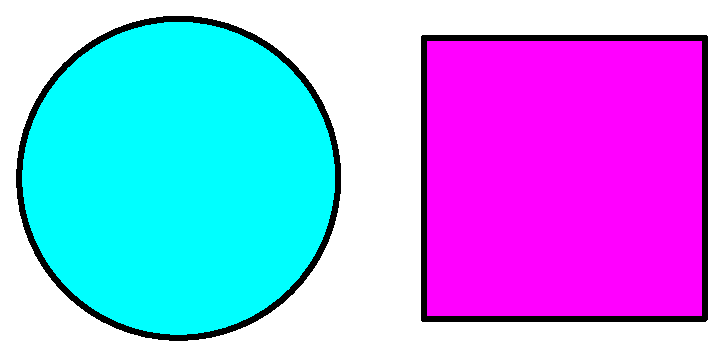
\includegraphics[width=7cm]{carre-et-cercle}
 \caption{Titre de la figure qui doit normalement se tenir sur deux lignes dans la liste des figures.}
 \label{fig:figure_long}
\end{figure}

On s'attend à ce que vos figures soient dans le dossier \verb+fig+. Remarquez que dans ce cas, vous n'avez pas besoin de donner le chemin de la figure (seulement son nom). De plus, on recommande de ne pas donner l'extension du fichier (\LaTeX{} devine tout seul s'il s'agit d'un PNG, PDF, JPG, etc.).

Vous pouvez ensuite mentionner la Figure \ref{fig:figure_long} dans votre texte.

\begin{figure}
  \centering
  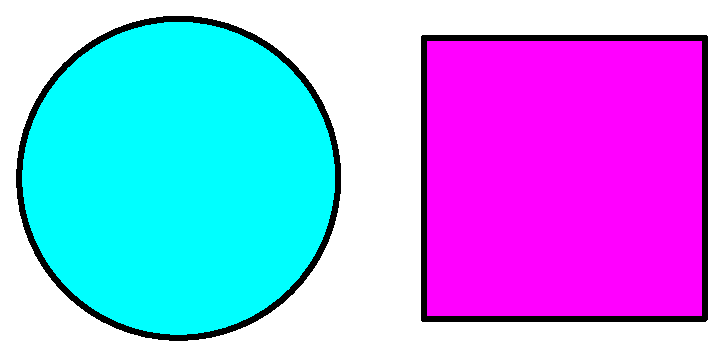
\includegraphics[width=7cm]{carre-et-cercle}
  \caption[Titre de la figure sans citation]{Titre de la figure qui comporte une citation de \citet{RN6}.}
  \label{fig:figure_cite}
 \end{figure}

Vous pouvez aussi référencer la Figure \ref{fig:figure_cite} directement dans votre texte.

\subsection{Tableaux}

On peut ajouter des tableaux au texte avec un environnement \verb+table+, qui inclut généralement un environnement \verb+tabular+. À noter que contrairement aux figures, la légende du tableau est au-dessus de celui-ci.

\begin{table}
\centering
\caption{Titre du tableau qui doit normalement se tenir sur deux lignes dans la liste des tableaux.}
\label{tab:tab_1}
\begin{tabular}{l|c|r}
  \textbf{Value 1} & \textbf{Value 2} & \textbf{Value 3}\\
  $\alpha$ & $\beta$ & $\gamma$ \\
  \hline
  1 & 1110.1 & a\\
  2 & 10.1 & b\\
  3 & 23.113231 & c\\
\end{tabular}
\end{table}

Vous pouvez ensuite mentionner le Tableau \ref{tab:tab_1} dans votre texte.

\subsection{Citations}

Exemples de citations: blabla la théorie des types
\cite{DBLP:journals/jsyml/Turing48,DBLP:journals/ai/Lenat82}. Si on mentionne
le nom, ne pas le répéter dans la citation: comme le disait
\citeauthor{DBLP:journals/jsyml/Turing48}, ou même
\citeauthor{DBLP:conf/afips/SolomonP76}.

\section{Une autre section}

Praesent diam libero, tincidunt vel interdum at, luctus id nisl. Ut egestas
nisi a elit ullamcorper tempus. Sed nisl enim, fermentum et consequat ac,
aliquam quis diam. Nulla elementum, purus nec fermentum vestibulum, justo
ligula tempus orci, non dignissim ligula orci id nulla. Integer placerat
posuere quam sit amet congue. Proin eleifend, turpis mollis gravida
tristique, justo nisl semper nunc, quis pellentesque neque ligula eu quam.
Cras a felis urna. Suspendisse dui sem, ullamcorper sed viverra a, varius id
odio. Nullam in nisi id massa tempor varius cursus id neque. Curabitur
ultrices fermentum purus tempor scelerisque. Maecenas in iaculis tellus.
Nulla et sollicitudin quam. Pellentesque sed mi at massa facilisis auctor.
Quisque non metus massa.

\subsection{Un sous-titre}

Fusce et dui at mi semper aliquam in sed ipsum. Etiam in urna enim.
Vestibulum arcu tellus, venenatis ac sollicitudin vel, sagittis eget nisl.
Mauris ut nunc ipsum. Phasellus ut magna a nisi aliquam scelerisque ut a
sapien. Ut lectus leo, faucibus vitae sagittis ac, sagittis posuere tortor.
Nulla id odio dui, eu pharetra massa. Etiam bibendum posuere elit, sit amet
tristique leo blandit sed. Voyez par exemple la figure \ref{fig:formes}.

\begin{figure}
  \begin{center}
  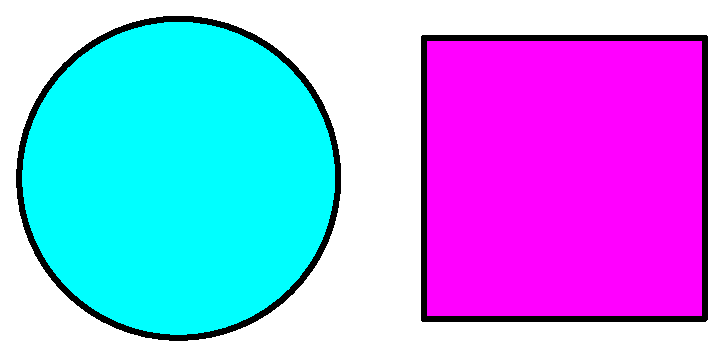
\includegraphics[width=3in]{carre-et-cercle}
  \end{center}
  \caption{Des formes géométriques}
  \label{fig:formes}
\end{figure}

Pellentesque molestie laoreet gravida. Curabitur egestas mollis libero, in
posuere turpis malesuada at. Donec egestas nunc sed justo eleifend
tincidunt. Vestibulum dignissim lobortis nisl, quis gravida tortor pulvinar
id. In ac nisi metus, in varius felis. Morbi semper aliquam turpis sed
vehicula. Nam neque libero, condimentum sed gravida ut, egestas ut nibh.
Lorem ipsum dolor sit amet, consectetur adipiscing elit.

\subsection{Un autre sous-titre}

Sed lacus mi, aliquet et elementum id, tincidunt in leo. Donec id ligula
erat, sit amet condimentum justo. Aliquam mi risus, molestie quis egestas
id, consequat nec erat. Aenean hendrerit augue quis massa consequat eu
ultricies lorem tincidunt. Lorem ipsum dolor sit amet, consectetur
adipiscing elit. Donec ornare ligula quis nunc tincidunt euismod. Phasellus
eget mi elit. Suspendisse neque est, placerat ac tincidunt ut, dapibus non
ante. Morbi varius, orci sed interdum euismod, risus purus dapibus magna,
non convallis augue augue eget elit. Comme le dit le tableau
\ref{tab:villes}. Duis ut feugiat massa. Duis at nunc non lacus rhoncus
porta vitae vel felis. Etiam eu euismod libero. Vestibulum ante ipsum primis
in faucibus orci luctus et ultrices posuere cubilia Curae; Fusce facilisis
dui eu augue ultrices non venenatis lectus viverra.

\begin{table}
  \caption{Un tableau avec un titre}
  \begin{center}
    \begin{tabular}{|c|c|c|}
      \hline
      Ville & Année & Naissance \\
      \hline\hline
      Chicoutimi & 2000 & 1936 \\
      \hline
      Jonquière & 2001 & 1944 \\
      \hline
      La Baie & 2002 & 1952 \\
      \hline
  \end{tabular}
  \label{tab:villes}
  \end{center}
\end{table}

\section{Une seconde section}

Curabitur quis arcu urna, sed laoreet magna. Proin ut sollicitudin arcu.
Suspendisse rhoncus, mauris sit amet lacinia interdum, justo erat auctor
nisi, at eleifend orci neque id ipsum. Aliquam rutrum accumsan dolor, sit
amet elementum mauris gravida vel. In hac habitasse platea dictumst. Mauris
sit amet diam velit, non rhoncus lorem. Suspendisse pulvinar, dolor a tempor
cursus, nibh nisl tincidunt augue, non aliquet mauris enim vitae massa.
Vestibulum ante ipsum primis in faucibus orci luctus et ultrices posuere
cubilia Curae; Suspendisse potenti. Nullam rutrum, dolor quis molestie
sollicitudin, ipsum orci condimentum nibh, nec tincidunt sem nisi eget leo.
Ut porta metus neque, id tincidunt est. Phasellus mollis porta euismod.

\[
  \sum_{i=0}^n i = \frac{n(n+1)}{2}
\]

Morbi pellentesque, urna in gravida porta, neque nisl imperdiet lorem, at
molestie lacus dolor aliquam eros. Duis vel interdum ante. Aenean dignissim,
dolor sed accumsan vulputate, elit ipsum mollis mauris, ultricies cursus
lorem enim sit amet elit. Suspendisse congue dolor vel urna semper at mattis
leo cursus. Phasellus cursus, odio ut gravida auctor, nisi lacus iaculis
erat, in interdum elit dolor et est. Nunc eleifend ullamcorper erat, lacinia
suscipit augue luctus vel. Etiam quis nisl vel turpis sodales bibendum vitae
ac velit. Pellentesque accumsan lacus massa. Nunc sollicitudin massa
adipiscing neque placerat vestibulum.

\subsection{Un sous-titre}

Quisque a lorem sit amet diam sollicitudin lobortis vitae ac massa. Mauris
id eros sed enim egestas eleifend at vel nunc. Vivamus risus erat, pretium
quis convallis sit amet, pellentesque id sem. Cras massa metus, luctus eu
molestie adipiscing, condimentum sit amet mauris. Sed euismod consectetur
blandit. Nunc et nunc sed nunc tempor aliquam. Class aptent taciti sociosqu
ad litora torquent per conubia nostra, per inceptos himenaeos. Vestibulum
rhoncus feugiat orci, non venenatis mauris lobortis quis. Aenean
sollicitudin tempor diam, at feugiat leo adipiscing ut. Vivamus fermentum
semper diam vitae ultrices. Nulla consequat ullamcorper nulla ac consequat.

\subsection{Un dernier sous-titre}

Duis sed augue et sem tempus tempor. Fusce ut bibendum diam. In orci tellus,
porttitor ut euismod porttitor, lacinia in lacus. Aenean augue sem, porta
eget ultricies id, ornare a purus. Nulla facilisi. Donec non dignissim
purus. Nam arcu velit, placerat ut convallis at, laoreet nec sem. Phasellus
ac nisl et tellus adipiscing varius. Phasellus consequat tristique est, at
mattis magna ullamcorper at. Donec bibendum, arcu ac scelerisque vulputate,
massa erat porta sapien, a iaculis erat ligula aliquam ligula. Nam eget elit
lacus. Donec vel arcu ut dolor consequat pretium. Suspendisse gravida
vestibulum arcu, sit amet viverra sem feugiat consequat. Aliquam ultrices
gravida condimentum. Sed turpis magna, blandit in porttitor quis, interdum
eu erat.

Etiam tincidunt arcu sed nulla adipiscing vel tempus erat luctus. Nulla
convallis hendrerit feugiat. Curabitur et vehicula ante. Mauris mattis enim
et lorem consectetur venenatis sollicitudin sapien pharetra. Nulla dictum
mattis tincidunt. Nullam urna ipsum, aliquet consequat semper eu, vestibulum
at dolor. Morbi libero tellus, dignissim ut elementum a, rutrum nec lacus.
Pellentesque id venenatis turpis. Pellentesque habitant morbi tristique
senectus et netus et malesuada fames ac turpis egestas. Nunc rutrum mollis
sodales. Cum sociis natoque penatibus et magnis dis parturient montes,
nascetur ridiculus mus. Fusce urna ante, facilisis sit amet posuere vitae,
interdum quis felis. Quisque sollicitudin, urna et vestibulum feugiat, elit
lectus egestas tellus, a ultrices nulla tellus mattis mi. Vivamus id tellus
ac quam aliquet vestibulum vehicula non dui.

%% :wrap=soft:
%! TeX root = these.tex
\chapter{Titre d'un chapitre}\label{chap:chap_2}

Lorem ipsum dolor sit amet, consectetur adipiscing elit. Nulla pellentesque ante ut velit tincidunt rhoncus. Ut aliquam consectetur tempor. Nulla luctus nisl at urna placerat tristique. Suspendisse tempus iaculis nisl at suscipit. Class aptent taciti sociosqu ad litora torquent per conubia nostra, per inceptos himenaeos. Nulla vel libero placerat enim scelerisque interdum quis nec tortor. Quisque fermentum rhoncus dolor sodales sollicitudin. Donec quis mi nisi, quis blandit nulla. Pellentesque varius ipsum ut tortor pretium vel eleifend diam iaculis. Aenean nulla ligula, congue in placerat non, varius ut nibh.

\section{Exemples avancés}

Suspendisse tempus iaculis nisl at suscipit. Class aptent taciti sociosqu ad litora torquent per conubia nostra, per inceptos himenaeos.

\subsection{Équations}

\begin{equation}
  \label{eq:eq_1}
  \sum_{i=0}^n i = \frac{n(n+1)}{2}
\end{equation}

Il est possible de référencer l'Équation \ref{eq:eq_1} dans le texte.

\subsection{Théorèmes et preuves}

Il faut d'abord définir les environnements.

\newtheorem{theorem}{Théorème}
\newtheorem{corollary}{Corollaire}
\newtheorem{lemma}{Lemme}
\newtheorem{definition}{Definition}
\newtheorem{proof}{Preuve}

\begin{theorem}
  \label{theo:theo_1}
  Soit $f$ une fonction dont la dérivée existe en chaque point, alors $f$
  est une fonction continue.
\end{theorem}

\begin{theorem}[Théorème de Pythagore]
  \label{theo:theo_2}
  C'est un théorème sur les triangles rectangles et peut se résumer par
  l'équation suivante
  \[ x^2 + y^2 = z^2 \]
\end{theorem}

\begin{corollary}
  \label{coro:coro_1}
  Il n'existe pas de triangle rectangle dont les côtés mesurent 3 cm, 4 cm, et 6 cm.
\end{corollary}

\begin{lemma}
  \label{lem:lem_1}
  Étant donné deux segments de longueur $a$ et $b$ respectivement, il existe un nombre réel $r$ tel que $b=ra$.
\end{lemma}

\begin{definition}[Fibration]
  \label{def:def_1}
  Une fibration est une application entre deux espaces topologiques qui possède la propriété de relèvement de l'homotopie pour tout espace $X$.
\end{definition}

\begin{proof}
  \label{proof:proof_1}
  Pour démontrer cela par contradiction, supposez que l'énoncé est faux,   procédez à partir de là et à un certain moment, vous arriverez à une contradiction.
\end{proof}

Vous pouvez ensuite référencer les théorèmes \ref{theo:theo_1} et \ref{theo:theo_2}, ainsi que le corollaire \ref{coro:coro_1} et le Lemme \ref{lem:lem_1} dans votre texte. De plus, la définition \ref{def:def_1} et la démonstration \ref{proof:proof_1} peuvent également être référencées dans le texte.

\subsection{Code source}

On peut inclure du code source avec un environment \verb+lstlisting+.

\begin{lstlisting}[caption=Exemple de code]
for (i=0; i < 10; ++i) {
  // code
}
\end{lstlisting}


%% :wrap=soft:
%% ...
%% Ajoutez autant de commandes include qu'il y a de chapitres à
%% inclure dans votre document
%% ...
%! TeX root = these.tex
\chapter{Conclusion}

Lorem ipsum dolor sit amet, consectetur adipiscing elit. Aenean ac
ullamcorper mi. Vivamus non turpis odio. Cras vel mauris mauris. Vivamus
augue justo, fringilla vitae placerat a, rutrum placerat mi. Mauris in
ligula in velit aliquam sodales eu ac est. Phasellus elementum interdum
lectus id congue. Nullam eget rutrum augue.

Quisque ut tellus nulla. Phasellus ut turpis quis erat semper pharetra.
Donec consectetur vehicula dui id pretium. In et massa lectus. Nulla mattis
pulvinar convallis. Etiam at odio velit. Phasellus eleifend, neque vel
euismod rutrum, turpis orci gravida velit, vel placerat arcu lectus quis
nisl. Vivamus vel mauris justo. Donec facilisis facilisis sem, in vestibulum
quam imperdiet eget. Sed tortor justo, adipiscing a tincidunt at, pharetra
vitae felis. Ut quis orci leo, id suscipit leo. Maecenas tincidunt lectus et
risus tempus non tristique libero tempor. In arcu sapien, suscipit ac tempor
eu, venenatis ut tellus. Nullam metus felis, tempor id scelerisque tempor,
fermentum non nisl. Nulla viverra ultricies neque sit amet facilisis.

%% ------------------------
%% Bibliograhpie
%% ------------------------
\backmatter

%% Liste des fichiers source pour la bibliograhpie.
%% On peut inclure plus d'un fichier en séparant leurs noms par des
%% virgules.
\phantomsection
\singlespacing
\SansBibliography{these}
\doublespacing

%% ------------------------
%% Annexes (le cas échéant)
%% ------------------------
\appendix
%! TeX root = these.tex
% Les annexes n'ont pas de numéro mais apparaissent dans la table des matières
\chapter*{Annexe A: Quelque chose à ajouter}

Lorem ipsum dolor sit amet, consectetur adipiscing elit. Aenean ac
ullamcorper mi. Vivamus non turpis odio. Cras vel mauris mauris. Vivamus
augue justo, fringilla vitae placerat a, rutrum placerat mi. Mauris in
ligula in velit aliquam sodales eu ac est. Phasellus elementum interdum
lectus id congue. Nullam eget rutrum augue.

Quisque ut tellus nulla. Phasellus ut turpis quis erat semper pharetra.
Donec consectetur vehicula dui id pretium. In et massa lectus. Nulla mattis
pulvinar convallis. Etiam at odio velit. Phasellus eleifend, neque vel
euismod rutrum, turpis orci gravida velit, vel placerat arcu lectus quis
nisl. Vivamus vel mauris justo. Donec facilisis facilisis sem, in vestibulum
quam imperdiet eget. Sed tortor justo, adipiscing a tincidunt at, pharetra
vitae felis. Ut quis orci leo, id suscipit leo. Maecenas tincidunt lectus et
risus tempus non tristique libero tempor. In arcu sapien, suscipit ac tempor
eu, venenatis ut tellus. Nullam metus felis, tempor id scelerisque tempor,
fermentum non nisl. Nulla viverra ultricies neque sit amet facilisis.

%% Décommenter cette ligne pour afficher l'index
% \printindex

\end{document}
%% Codes pour jEdit
%% :mode=latex:wrap=none: